\documentclass[tikz]{standalone}\usepackage[]{graphicx}\usepackage[]{xcolor}
% maxwidth is the original width if it is less than linewidth
% otherwise use linewidth (to make sure the graphics do not exceed the margin)
\makeatletter
\def\maxwidth{ %
  \ifdim\Gin@nat@width>\linewidth
    \linewidth
  \else
    \Gin@nat@width
  \fi
}
\makeatother

\definecolor{fgcolor}{rgb}{0.345, 0.345, 0.345}
\newcommand{\hlnum}[1]{\textcolor[rgb]{0.686,0.059,0.569}{#1}}%
\newcommand{\hlsng}[1]{\textcolor[rgb]{0.192,0.494,0.8}{#1}}%
\newcommand{\hlcom}[1]{\textcolor[rgb]{0.678,0.584,0.686}{\textit{#1}}}%
\newcommand{\hlopt}[1]{\textcolor[rgb]{0,0,0}{#1}}%
\newcommand{\hldef}[1]{\textcolor[rgb]{0.345,0.345,0.345}{#1}}%
\newcommand{\hlkwa}[1]{\textcolor[rgb]{0.161,0.373,0.58}{\textbf{#1}}}%
\newcommand{\hlkwb}[1]{\textcolor[rgb]{0.69,0.353,0.396}{#1}}%
\newcommand{\hlkwc}[1]{\textcolor[rgb]{0.333,0.667,0.333}{#1}}%
\newcommand{\hlkwd}[1]{\textcolor[rgb]{0.737,0.353,0.396}{\textbf{#1}}}%
\let\hlipl\hlkwb

\usepackage{framed}
\makeatletter
\newenvironment{kframe}{%
 \def\at@end@of@kframe{}%
 \ifinner\ifhmode%
  \def\at@end@of@kframe{\end{minipage}}%
  \begin{minipage}{\columnwidth}%
 \fi\fi%
 \def\FrameCommand##1{\hskip\@totalleftmargin \hskip-\fboxsep
 \colorbox{shadecolor}{##1}\hskip-\fboxsep
     % There is no \\@totalrightmargin, so:
     \hskip-\linewidth \hskip-\@totalleftmargin \hskip\columnwidth}%
 \MakeFramed {\advance\hsize-\width
   \@totalleftmargin\z@ \linewidth\hsize
   \@setminipage}}%
 {\par\unskip\endMakeFramed%
 \at@end@of@kframe}
\makeatother

\definecolor{shadecolor}{rgb}{.97, .97, .97}
\definecolor{messagecolor}{rgb}{0, 0, 0}
\definecolor{warningcolor}{rgb}{1, 0, 1}
\definecolor{errorcolor}{rgb}{1, 0, 0}
\newenvironment{knitrout}{}{} % an empty environment to be redefined in TeX

\usepackage{alltt}

\usepackage{tikz}
\IfFileExists{upquote.sty}{\usepackage{upquote}}{}
\begin{document}

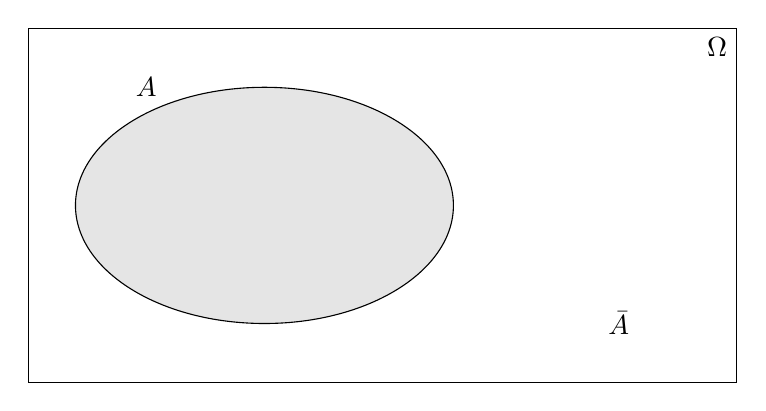
\begin{tikzpicture}[scale=3]
  \draw     (1.5,.75) node[below left] {$\Omega$}; 
  \draw     (-1.5,-.75) rectangle (1.5,.75); 
  \draw    [fill=gray!20] (-.5,0) ellipse (.8 and .5); 
  \draw     (-1,.5) node {$A$}; 
  \draw     ( 1,-.5) node {$\bar{A}$}; 
\end{tikzpicture}

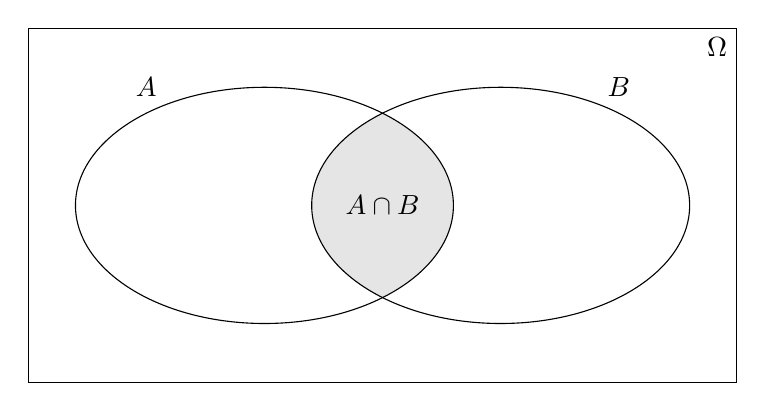
\begin{tikzpicture}[scale=3]
    \draw     (1.5,.75) node[below left] {$\Omega$};
    \draw     (-1.5,-.75) rectangle (1.5,.75);
    \begin{scope}
        \clip     (-.5,0) ellipse (.8 and .5);
        \clip    ( .5,0) ellipse (.8 and .5);
        \filldraw[color=gray!20]    (-2,1.5) rectangle (2,-1.5);
    \end{scope}
    \draw     (-.5,0) ellipse (.8 and .5);
    \draw     ( .5,0) ellipse (.8 and .5);
    \draw     (0,0) node {$A\cap B$};
    \draw     (-1,.5) node {$A$};
    \draw     ( 1,.5) node {$B$};
\end{tikzpicture}

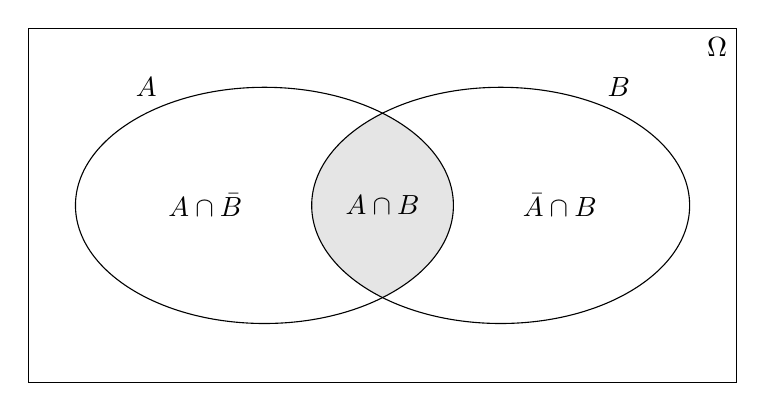
\begin{tikzpicture}[scale=3]
    \draw     (1.5,.75) node[below left] {$\Omega$};
    \draw     (-1.5,-.75) rectangle (1.5,.75);
    \begin{scope}
        \clip     (-.5,0) ellipse (.8 and .5);
        \clip    ( .5,0) ellipse (.8 and .5);
        \filldraw[color=gray!20]    (-2,1.5) rectangle (2,-1.5);
    \end{scope}
    \draw     (-.5,0) ellipse (.8 and .5);
    \draw     ( .5,0) ellipse (.8 and .5);
    \draw     (0,0) node {$A\cap B$};
    \draw     (-.75,0) node {$A\cap \bar B$};
    \draw     (+.75,0) node {$\bar A\cap B$};
    \draw     (-1,.5) node {$A$};
    \draw     ( 1,.5) node {$B$};
\end{tikzpicture}

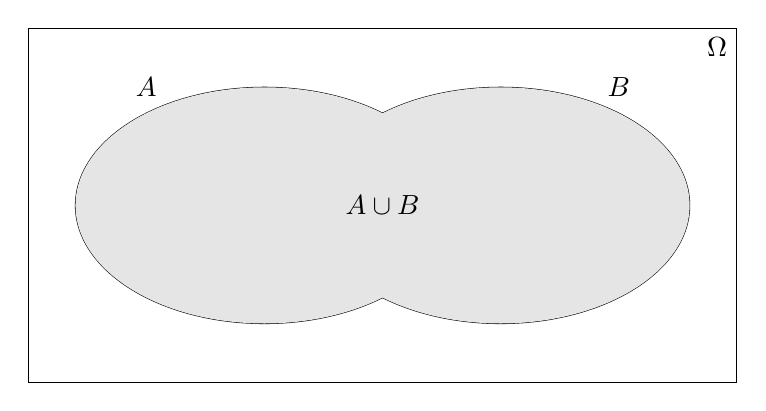
\begin{tikzpicture}[scale=3]
    \draw     (1.5,.75) node[below left] {$\Omega$};
    \draw     (-1.5,-.75) rectangle (1.5,.75);
    \fill[gray!20]    (-.5,0) ellipse (.8 and .5);
    \fill[gray!20]    ( .5,0) ellipse (.8 and .5);
    \draw    (-.5,0) ellipse (.8 and .5);
    \draw    ( .5,0) ellipse (.8 and .5);
    \fill[gray!20]   (-.5,0) ellipse (.8 and .5);
    \fill[gray!20]   ( .5,0) ellipse (.8 and .5);
    \draw     (0,0) node {$A\cup B$};
    \draw     (-1,.5) node {$A$};
    \draw     ( 1,.5) node {$B$};
\end{tikzpicture}

\begin{tikzpicture}[scale=3]
    \draw    (1.5,.75) node[below left] {$\Omega$};
    \draw    (-1.5,-.75) rectangle (1.5,.75);
    % \fill[white]    (-.6,0) ellipse (.8 and .5);
    % \fill[white]      ( .6,0) ellipse (.8 and .5);
    \draw    (-.6,0) ellipse (.55 and .35);
    \draw    ( .6,0) ellipse (.55 and .35);
    \draw    (-1,.5) node {$A$};
    \draw    ( 1,.5) node {$B$};
\end{tikzpicture}

% \begin{tikzpicture}[scale=3]
%     \draw    (1.5,1) node[below left] {$\Omega$};
%     \draw    (-1.5,-1) rectangle (1.5,1);
%     \fill[gray!20]    (-.5,0) ellipse (.8 and .5);
%     \fill[white]      ( .5,0) ellipse (.8 and .5);
%     \draw    (-.8,0) node {$A\setminus B$};
%     \draw    (-.5,0) ellipse (.8 and .5);
%     \draw    ( .5,0) ellipse (.8 and .5);
%     \draw    (-1,.5) node {$A$};
%     \draw    ( 1,.5) node {$B$};
% \end{tikzpicture}

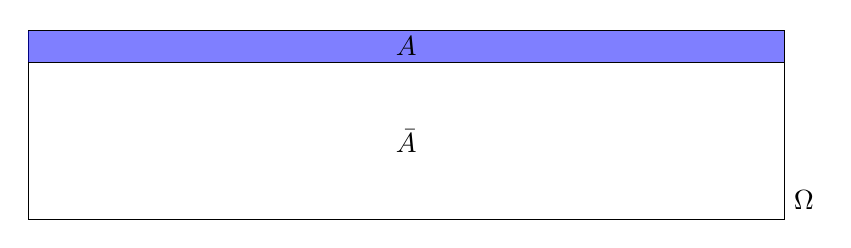
\begin{tikzpicture}[yscale=.2,xscale=.8]
      \draw (0,0) rectangle (12,12);
      \draw (12,0) node[anchor = south west] {$\Omega$};
      \fill[semitransparent,blue] (0,10) rectangle (12,12);
      \draw ( 0,10) -- (12,10);
      \draw ( 6,11) node  {$A$};
      % \fill[semitransparent,yellow] (0,10) rectangle (12,0);
      \draw ( 6, 5) node  {$\bar{A}$};
\end{tikzpicture}

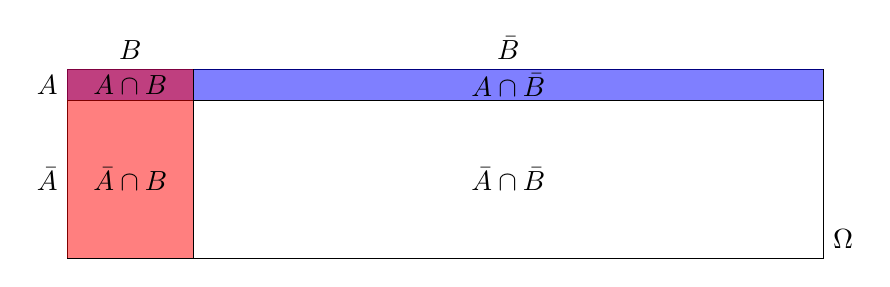
\begin{tikzpicture}[yscale=.2,xscale=.8]
        \draw (0,0) rectangle (12,12);
        \draw (12,0) node[anchor = south west] {$\Omega$};
        \fill[semitransparent,blue] (0,10) rectangle (12,12);
        \draw ( 0,10) -- (12,10);
        \draw ( 0,11) node[anchor =east]  {$A$};
        \draw ( 0, 5) node[anchor =east]  {$\bar{A}$};
        \fill[semitransparent,red] (0,0) rectangle (2,12);
        \draw ( 2,0) -- ( 2,12);
        \draw ( 1,12) node[anchor = south]  {$B$};
        \draw ( 7,12) node[anchor = south]  {$\bar{B}$};
        \draw ( 1, 5) node {$\bar{A}\cap B$};
        \draw ( 1,11) node {$A\cap B$};
        \draw ( 7, 5) node {$\bar{A}\cap \bar{B}$};
        \draw ( 7,11) node {$A\cap \bar{B}$};
\end{tikzpicture}

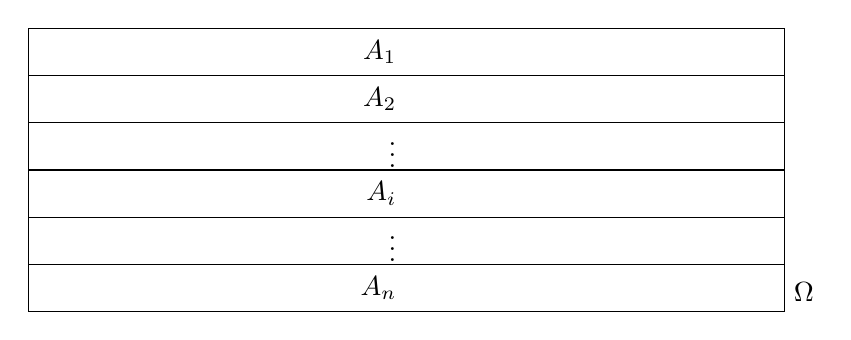
\begin{tikzpicture}[yscale=.3,xscale=.8]
        \draw (0,0) rectangle (12,12);
        \draw (12,0) node[anchor = south west] {$\Omega$};
        \draw ( 0,2) -- ( 12,2);
        \draw ( 0,4) -- ( 12,4);
        \draw ( 0,6) -- ( 12,6);
        \draw ( 0,8) -- ( 12,8);
        \draw ( 0,10) -- (12,10);
        \draw ( 6,1) node[anchor = east]   {$A_n$};
        \draw ( 6,3) node[anchor = east]   {$\vdots$};
        \draw ( 6,5) node[anchor = east]   {$A_i$};
        \draw ( 6,7) node[anchor = east]   {$\vdots$};
        \draw ( 6,9) node[anchor = east]   {$A_2$};
        \draw ( 6,11) node[anchor =east]  {$A_1$};
\end{tikzpicture}

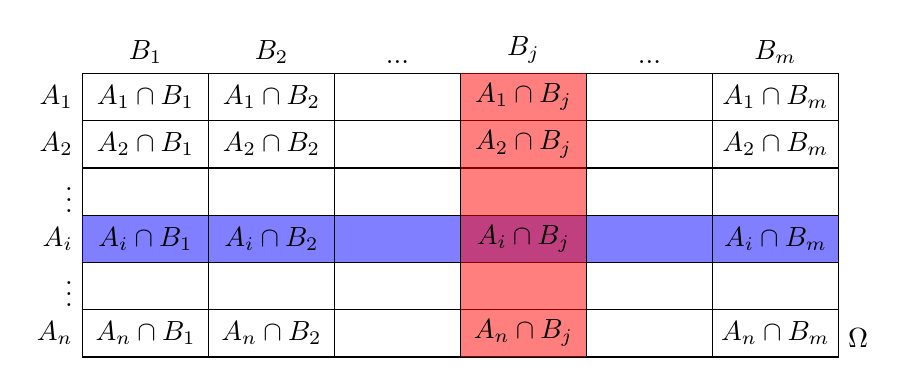
\begin{tikzpicture}[yscale=.3,xscale=.8]
      \draw (0,0) rectangle (12,12);
      \draw (12,0) node[anchor = south west] {$\Omega$};
      \fill[semitransparent,blue] (0,4) rectangle (12,6);
      \draw ( 0,2) -- ( 12,2);
      \draw ( 0,4) -- ( 12,4);
      \draw ( 0,6) -- ( 12,6);
      \draw ( 0,8) -- ( 12,8);
      \draw ( 0,10) -- (12,10);
      \draw ( 0,1) node[anchor = east]   {$A_n$};
      \draw ( 0,3) node[anchor = east]   {$\vdots$};
      \draw ( 0,5) node[anchor = east]   {$A_i$};
      \draw ( 0,7) node[anchor = east]   {$\vdots$};
      \draw ( 0,9) node[anchor = east]   {$A_2$};
      \draw ( 0,11) node[anchor =east]  {$A_1$};
      \fill[semitransparent,red] (6,0) rectangle (8,12);
      \draw ( 2,0) -- ( 2,12);
      \draw ( 4,0) -- ( 4,12);
      \draw ( 6,0) -- ( 6,12);
      \draw ( 8,0) -- ( 8,12);
      \draw (10,0) -- (10,12);
      \draw ( 1,12) node[anchor = south]  {$B_1$};
      \draw ( 3,12) node[anchor = south]  {$B_2$};
      \draw ( 5,12) node[anchor = south]  {$...$};
      \draw ( 7,12) node[anchor = south]  {$B_j$};
      \draw ( 9,12) node[anchor = south]  {$...$};
      \draw (11,12) node[anchor = south]   {$B_m$};
      \draw ( 1, 1) node {$A_n\cap B_1$};
      \draw ( 1, 5) node {$A_i\cap B_1$};
      \draw ( 1, 9) node {$A_2\cap B_1$};
      \draw ( 1,11) node {$A_1\cap B_1$};
      \draw ( 3, 1) node {$A_n\cap B_2$};
      \draw ( 3, 5) node {$A_i\cap B_2$};
      \draw ( 3, 9) node {$A_2\cap B_2$};
      \draw ( 3,11) node {$A_1\cap B_2$};
      \draw ( 7, 1) node {$A_n\cap B_j$};
      \draw ( 7, 5) node {$A_i\cap B_j$};
      \draw ( 7, 9) node {$A_2\cap B_j$};
      \draw ( 7,11) node {$A_1\cap B_j$};
      \draw (11, 1) node {$A_n\cap B_m$};
      \draw (11, 5) node {$A_i\cap B_m$};
      \draw (11, 9) node {$A_2\cap B_m$};
      \draw (11,11) node {$A_1\cap B_m$};
\end{tikzpicture}

\end{document}
